\subsection{System Identification using Dead-Time and PT1 elements}
\label{sec:ident_Tt_PT1}

It  is  known  that the motor has a dead-time built in, and by looking at  the
step  response, one can say that it looks like a PT1 element might be  a  good
approximation.

The dead time element and its Laplace transform is:

\begin{equation}
    F_{T_t}(s) = \laplace{\{\epsilon(t)(t-T_t)} = e^{-sT_t}\}
\end{equation}

The PT1 lag element and its Laplace transform is:

\begin{equation}
    F_{PT1}(s) = \laplace{\{\epsilon(t)e^{-sT_g}}\}
\end{equation}

These two elements are combined to obtain the model we will use to approximate
the measured step response:

\begin{equation}
    G_1(s) = F_1(s) \cdot F_2(s) = e^{-sT_t} \frac{K_s}{sT_g+1}
\end{equation}

By  plugging  in  the  parameters  obtained  from the characterisation step in
section  \ref{sec:sim:characterisation}  (dead-time  $T_t=T_u$)  we obtain the
following transfer function:

\begin{equation}
    G_1(s) = e^{-0.165*s}\frac{24.68}{5.96s + 1}
\end{equation}

Figure  \ref{fig:Tt_PT1_step}  shows  the  step  response  of  the  calculated
transfer function $G_1(s)$ and compares it to the measured step response. It's
pretty  close, perhaps the parameter $T_g$ can be adjusted so it rises faster.
When doing this, however, the function no longer matches  the measured data at
the  beginning  where  it  starts  rising.  It's  possible therefore that  the
measured system  is of higher order. Adding more PT1 elements to our model can
help make the approximation more  exact, but for this experiment we will stick
to a single PT1 element.

By  looking  at  the  Bode-Diagram  of  the   model   $G_1(s)$   (see   figure
\ref{fig:Tt_PT1_bode})  it  is  very  easy  to  determine  the  critical  gain
$K_{s,crit}$. This is the  point at which the phase exceeds \SI{180}{\degree}.
The amplitude at  this  point  is  about  \SI{-36}{\decibel}, which means that
$K_{s,crit}=\SI{36}{\decibel}$, or:

\begin{equation}
    K_{s,crit} = 10^{\frac{\SI{36}{\decibel}}{20}} \approx 63.1
\end{equation}

\begin{figure}[h]
    \centering
    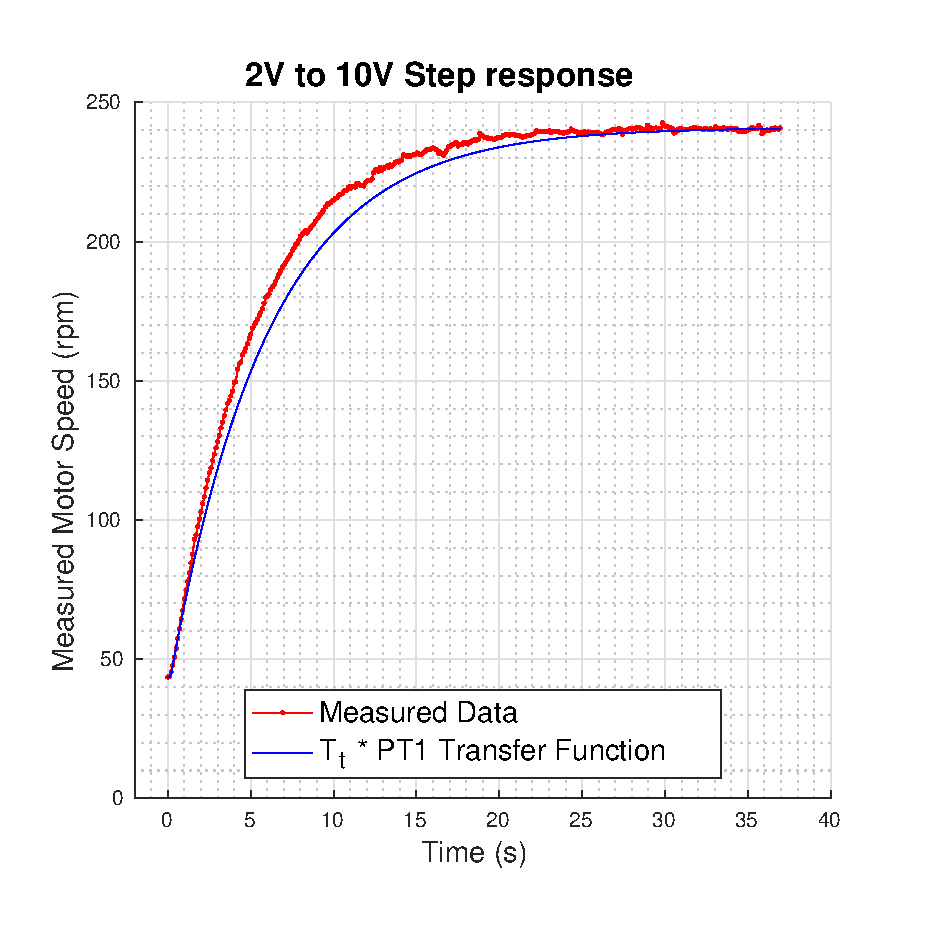
\includegraphics[width=\imagewidth]{images/Tt_PT1}
    \caption{Step response comparison of calculated system $G_1(s)$ and the measured step response.}
    \label{fig:Tt_PT1_step}
\end{figure}

The  closed  loop  transfer  function  of  $G_1(s)$  with  a  P-controller  is
constructed:

\begin{equation}
    T(s) = \frac{H(s)G_1(s)}{1 + H(s)G_1(s)}
\end{equation}

Where  $H(s)$  is  simply  the  P controller. By setting $H(s)=K_{p,crit}$ and
simulating a step  response,  we  obtain  a  system  that exhibits an undamped
oscillation (see  figure \ref{fig:Tt_PT1_tcrit}). Determining $\tau_{crit}$ is
now simply a matter of measuring two points in this graph.

\begin{equation}
    \tau_{crit} \approx 0.66
\end{equation}

\begin{figure}[h]
    \centering
    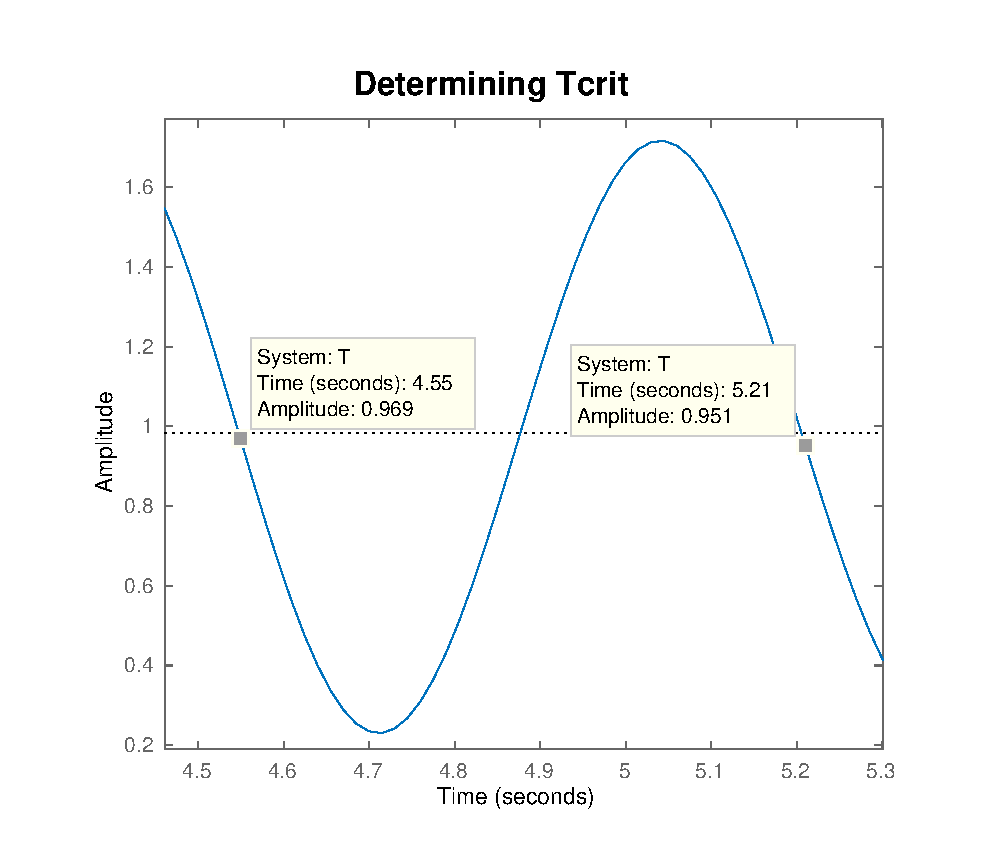
\includegraphics[width=\imagewidth]{images/tcrit}
    \caption{Step response of the closed loop transfer function with $K_p=K_{p,crit}$}
    \label{fig:Tt_PT1_tcrit}
\end{figure}

\begin{figure}[h]
    \centering
    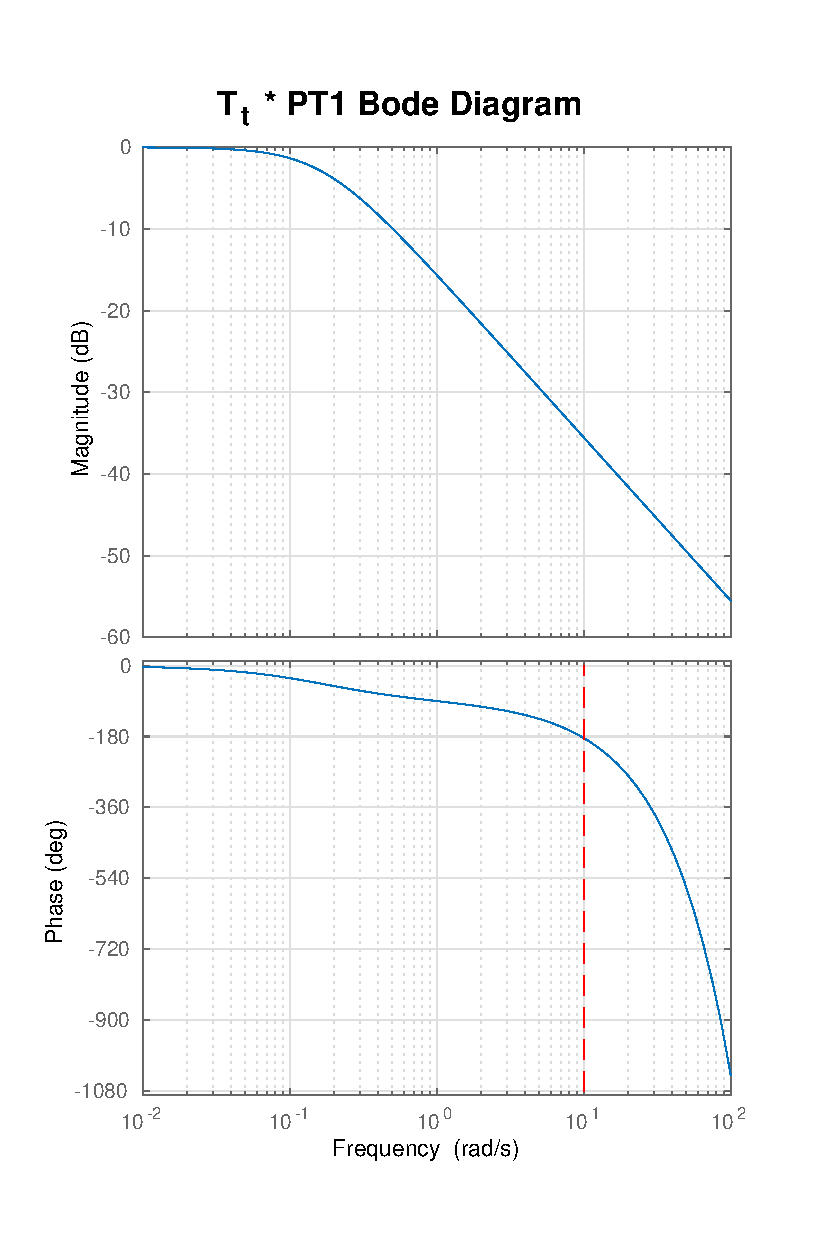
\includegraphics[width=\imagewidth]{images/Tt_PT1_bode}
    \caption{Bode-Plots of the model $G_1(s)$. The phase exceeds \SI{180}{\degree} at about \SI{-36}{\decibel}}
    \label{fig:Tt_PT1_bode}
\end{figure}

